\chapter{k-Selection Optimization in RAG }
\pagestyle{fancy}\lhead{\textbf \footnotesize\it{k-Selection Optimization in RAG }}
\pagestyle{fancy}\chead{} \pagestyle{fancy}\rhead{} 
\pagestyle{fancy}\cfoot{} \pagestyle{fancy}\rfoot{\thepage}
%%%%%%%%%%%%%%%%%%%%%%%%%%%%%%%%%%%%%%%%
\section{Introduction}
Retrieval-Augmented Generation systems enhance language models by grounding responses in externally retrieved documents. A critical challenge is determining the optimal number of documents k to retrieve for a given query. In this chapter, we first explore methods, highlighting their strengths and limitations We then introduce our novel hybrid dynamic selection algorithm provide detailed description of its methodology and present experimental results that demonstrate the effectiveness of its performance . 

\section{Defining k: The Number of Retrieved Documents}
the parameter k denotes the number of documents or passages retrieved from an external knowledge base. This retrieval process is managed by the retriever component\citep{pareto2024rag},which identifies the top k relevant documents based on similarity to the query typically using embedding-based search\citep{Rossi_2024} (e.g., dense retrieval with FAISS, BM25, or hybrid methods) Subsequently, these documents are passed to the generator, typically a language model, which synthesizes the final response by integrating the retrieved 
\begin{figure}[h]
	\centering
	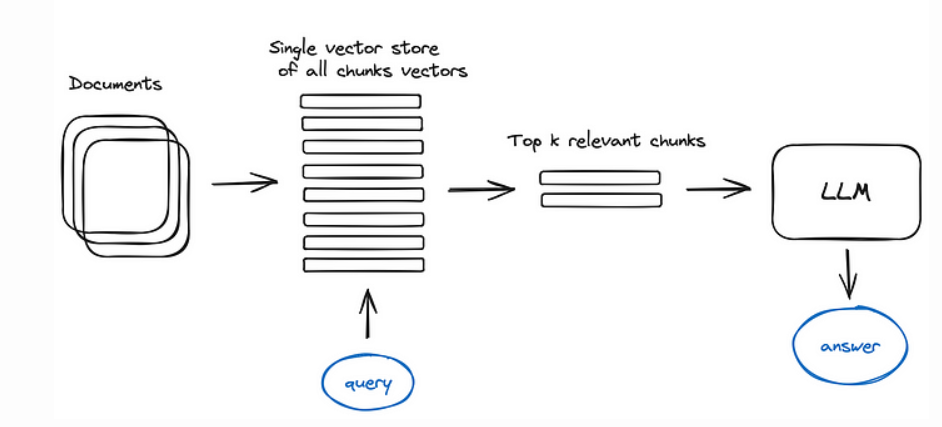
\includegraphics[width=0.9\linewidth]{Figures/topk.png}
	\caption{Basic retrieval}
	\label{rag_retrival.png}
	
\end{figure}

\section{Impact of k on Retrieval Performance}
The retriever's effectiveness in identifying relevant documents depends on k. Key impacts include :
\subsection{Recall vs. Precision} 
When a user conducts a search query, the outcomes from the database can be grouped into four distinct types based on relevance and retrieval status \citep{geeksforgeeks2022precision}:
\begin{itemize}
	\item {Relevant and Retrieved:} Documents that both address the user’s query and appear in the search results.
	\item {Relevant and Not Retrieved:} Useful documents that answer the query but are not included in the results.
	
	\item {Non-Relevant and Retrieved:} Documents that appear in the results but lack meaningful value for the query.
	 
	\item {Non-Relevant and Not Retrieved:} Irrelevant documents excluded from the results.
\end{itemize}


\textbf{Precision@k}: evaluates the proportion of relevant documents within the top k retrieved results. This metric is particularly valuable in scenarios where the focus is on delivering highly relevant information quickly, rather than ensuring complete coverage such as ,recommendation systems or search engines\citep{deconvoluteai2024metrics}.
\begin{equation}
\text{Precision@k} = \frac{\text{Number of Relevant Items Retrieved in Top k}}{k}
\end{equation}
\textbf{Example}
Suppose we have a dataset of 10 documents. If we retrieve \( k = 4 \) documents and find that 3 of them are relevant to the query:

\begin{itemize}
	\item \textbf{Dataset}: [doc1, doc2, doc3, doc4, doc5, doc6, doc7, doc8, doc9, doc10]
	\item \textbf{Retrieved}: [doc3, doc1, doc7, doc4]
	\item \textbf{Relevant}: [doc1, doc3, doc5, doc8]
\end{itemize}

The Precision@4 score would be:

\begin{equation}
\text{Precision@4} = \frac{3}{4} = 0.75
\end{equation}


\textbf{Recall@k :}Evaluates the proportion of relevant documents that are successfully retrieved within the top k results. This metric is particularly important in contexts where ensuring the completeness of information is crucial, such as in medical research or academic tools, where omitting relevant documents could result in incomplete or inaccurate conclusions\citep{deconvoluteai2024metrics}.
\begin{equation}
\text{Recall@k} = \frac{\text{Number of Relevant Items Retrieved in Top k}}{\text{Total Number of Relevant Items}}	
\end{equation}
\textbf{Example:}
Consider a dataset of 10 documents. If we retrieve \( k = 4 \) documents and find that 2 of them are relevant, while the total number of relevant documents in the dataset is 4
\begin{equation}
\text{Recall@4} = \frac{2}{4} = 0.5
\end{equation}
Increasing k typically enhances recall by retrieving more relevant documents but may decrease precision due to the inclusion of irrelevant ones. Conversely, decreasing k can improve precision but at the cost of lower recall. 
\subsection{Retrieval Speed and Computational Cost}
Retrieval speed and computational cost are two important areas where k has a big influence Below is a detailed explanation of how higher k values affect these aspects.

\textbf{Increased Computational Resources:} \\
As the value of k expands, the retrieval must handle a larger set of documents, leading to higher computational demands. Specifically, the system needs to perform additional operations like ranking, filtering, and similarity scoring to identify the most relevant documents. These tasks become increasingly resource-intensive, particularly in large-scale retrieval settings where the document corpus consists of millions or even billions of entries\citep{manning2008ir}. For instance, retrieving the top  documents (k=80) requires significantly more computational resources compared to retrieving only the top 10 documents (k=5). 

\textbf{Higher Memory Usage:}
As the number of retrieved documents k increases, Storing and processing a larger set of retrieved documents requires more memory This can become a significant bottleneck, especially in environments with constrained memory resources.

For large-scale retrieval tasks, where datasets may contain millions or even billions of documents, the memory demand grows proportionally with k. Each retrieved document needs to be stored temporarily, along with its associated metadata, such as embedding vectors, BM25 scores, or other relevance signals. Additionally, sorting and filtering operations further contribute to memory overhead
\subsection{Document Ranking Quality}
Document ranking in information retrieval involves ordering documents by their relevance to a user's query. The objective is to prioritize the most relevant documents at the top of search results, making it easier for users to access useful information quickly. Different models,Vector Space, including Boolean, and Probabilistic models, are used to establish this ranking \citep{enwiki:1262179867}.\\

Increasing the number of retrieved documents,represented as k, may result in the addition of lower-ranked, less relevant documents, potentially diluting the overall quality of the retrieved information. This occurs because of the inherent balance between precision and recall in information retrieval systems.
\begin{figure}[h]
	\centering
	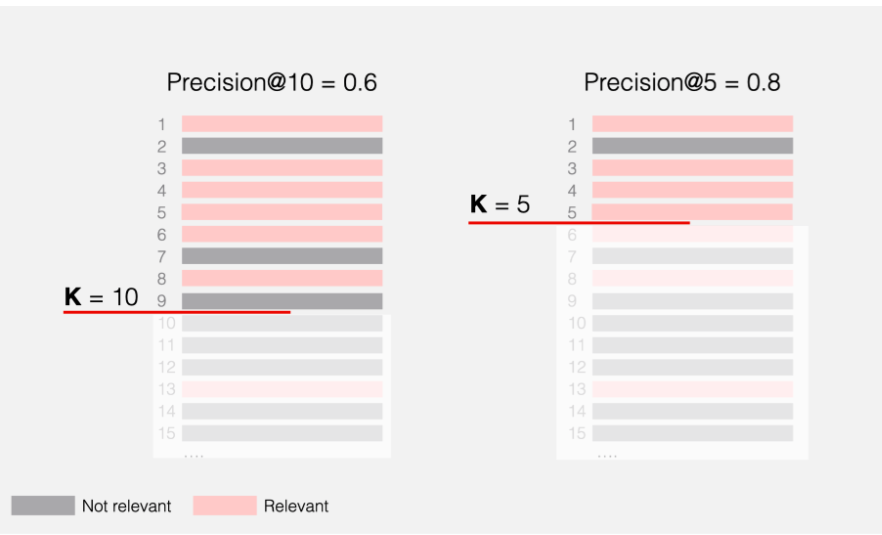
\includegraphics[width=0.7\linewidth]{Figures/precisionR.png}
	\caption{Precision in Document Ranking}
	\label{precisionR}
	
\end{figure}

\begin{figure}[h]
	\centering
	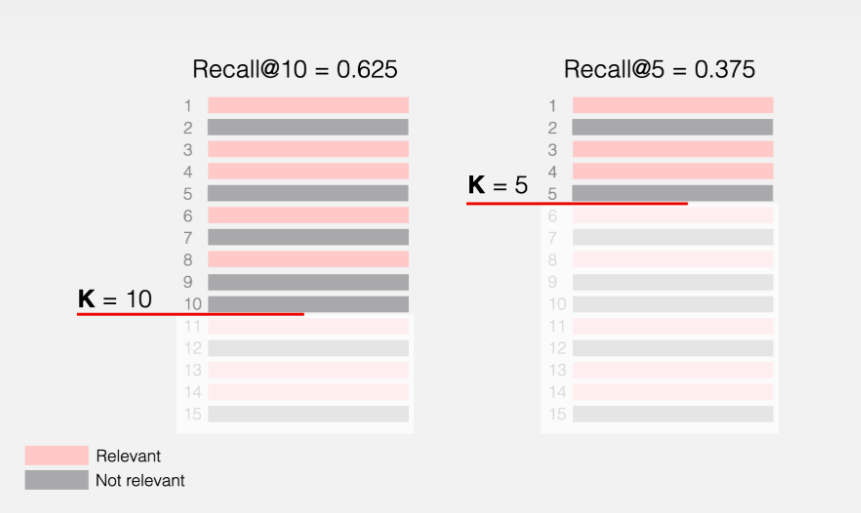
\includegraphics[width=0.7\linewidth]{Figures/recalR.png}
	\caption{Recall in Document Ranking}
	\label{recalR}
	
\end{figure}
As k grows, recall generally improves since a larger number of relevant documents are likely to be retrieved as shown in Figure \ref{recalR}. However, this often comes at the expense of precision, as the additional documents retrieved may include non-relevant ones, thereby lowering the overall precision as illustrated in Figure \ref{precisionR}. This trade-off is a core principle in evaluating information retrieval systems.

\section{Impact of k on Generation Quality}
The impact of k (the number of retrieved documents or generated candidates) on generation quality is A crucial factor in many machine learning and information retrieval tasks, including text generation, recommendation systems, and search engines. 

\subsection{Trade-off Between Diversity and Relevance} 
\textbf{Higher k:} Increasing k often improves diversity in generated outputs or retrieved documents, as more candidates are considered. However, this can lead to a drop in relevance or quality, as lower-ranked candidates may be less accurate or coherent. \\
\textbf{Lower k:} A smaller k tends to prioritize high-quality, relevant outputs but may lack diversity, leading to repetitive or overly narrow results.

Research shows that the quality of retrieved documents plays a crucial role in the performance of RAG . For example, one study demonstrated that the precision of retrieved documents directly affects the factual correctness of the generated responses \citep{salemi2023evaluating}
Additionally, another study \citep{wan2025cognitivealigneddocumentselectionretrievalaugmented} revealed that simply increasing the number of documents does not necessarily improve generation quality, especially if the additional documents are not highly relevant.
\subsection {Effect on Text Generation Models}
In text generation tasks, such as machine translation and dialogue systems, The parameter k frequently refers to the beam width in beam search algorithms\citep{freitag-al-onaizan-2017-beam}.Beam search is a heuristic search algorithm that expands the most promising nodes in a graph to maximize the quality of the text that is produced. Adjusting the beam width k has significantly impacts how well text generation models function.

As the beam width is increased, the model must process and retain more candidate sequences concurrently, leading to higher computational and memory demands Particularly in real-time applications where latency is crucial\citep{tensorrt_llm_beam_search}, this increase may have an effect on system performance and response time.

\section{Existing Solutions for k Selection}
Selecting an optimal k plays a crucial role in balancing retrieval effectiveness and generation quality. Over the years, various strategies have been proposed to determine k, ranging from static selection to dynamic and hybrid approaches.
\subsection{Static k Selection}
In RAG, "static k selection", refers to the process of setting a fixed number of top documents k to retrieve for every query, irrespective of how simple or complex the query might be. This approach simplifies the retrieval process by maintaining a consistent retrieval count across all queries.

\subsubsection{Sparse Retrieval with Fixed k} 
Sparse retrieval is a method of finding relevant documents from a large collection by representing both queries and documents as vectors where most values are zero\citep{zheng2024enhancing}. This focus on only the most important terms leads to faster, more accurate searches, especially useful when combining information from different sources 
Common approaches include. \textbf{BM25}\citep{10.1561/1500000019} where documents are scored for relevance by considering term frequency and inverse document frequency, it selects the k documents with the highest BM25 scores for each query,\textbf{TF-IDF} (Term Frequency-Inverse Document Frequency)\citep{gfg2025tfidf}in this method the retrieved documents would be those with the highest weighted term importance, Other methods like \textbf{QLM }(Query Likelihood Model)\citep{10.1007/978-3-030-72240-1_49}use probabilistic models to evaluate the likelihood of a query and rank documents according to textual similarity.

\subsubsection{Dense Retrieval with Fixed k} 
Dense retrieval \citep{karpukhin2020dense} is a method for retrieving information that uses deep learning models to convert documents and queries into high-dimensional vector embeddings, a fixed number of top-k documents are selected based on similarity scores between the query embedding and document embeddings in a continuous vector space, the retrieval process allows the system to capture semantic elationships beyond exact term matches.

Methods such as dual-encoder architectures (e.g., DPR - Dense Passage Retrieval)\citep{chen-etal-2024-dense} utilize separate neural networks (encoders) for queries and documents enable efficient retrieval, while Approximate Nearest Neighbor (ANN) search techniques (e.g., FAISS)\citep{enwiki:1276232158} optimize search efficiency in large-scale datasets .
\subsection{Dynamic k Selection}
In retrieval, dynamic k selection is the process of varying the quantity of documents k that are retrieved according to the properties of the query, such as its ambiguity, complexity, or relevance score distribution. This approach is crucial for enhancing the effectiveness and efficiency of information retrieval systems.

\subsubsection{Dynamic Trade-Off Prediction in Multi-Stage Retrieval Systems } This approach predicts the optimal number of documents k to retrieve. It uses pre-retrieval features to balance the trade-off between retrieval efficiency and effectiveness, ensuring that the system retrieves an appropriate number of documents for each query\citep{culpepper2016dynamictradeoffpredictionmultistage}.

\subsubsection{Dynamic Pruning Methods:}
This approach addresses the challenge of balancing effectiveness and efficiency in large-scale Information Retrieval systems, particularly under temporal constraints. The goal is to process queries within a specified time limit while minimizing the loss in retrieval effectiveness.\citep{10.1007/978-3-319-70145-5_1} The authors propose and evaluate three techniques for temporally constrained top-K query processing .
\subsection{Hybrid k Selection}
hybrid methods aim to achieve optimal retrieval By merging static and dynamic k selection, These methods balance computational efficiency (from static k) with adaptive flexibility (from dynamic k) ensuring high-quality retrieval Below are some key hybrid strategies.

\subsubsection{Blended RAG} 
An innovative method to improve Retrieval-Augmented Generation systems, which integrate private document collections with Large Language Models for Generative Question-Answering it employs a hybrid retrieval approach, combining Dense Vector indexes and Sparse Encoder indexes with sophisticated query strategies\citep{sawarkar2024blendedragimprovingrag}., Blended RAG provides a scalable and efficient solution for enhancing RAG, showcasing the effectiveness of merging dense and sparse retrieval techniques.

\subsubsection{ STAYKATE (Static-Dynamic Hybrid Selection)}
A new approach for selecting in-context examples to improve the performance of LLMs in scientific information extraction. Scientific tasks often struggle with limited training data and expensive annotation processes. STAYKATE tackles these challenges by merging static and dynamic selection strategies \citep{zhu2024staykatehybridincontextexample}, combining representativeness sampling from active learning with retrieval-based methods. This hybrid approach ensures the selection of high-quality, informative examples, enhancing in-context learning for LLMs.
\section{Proposed Solution}
While existing k-selection approaches—static, dynamic, and hybrid—offer distinct advantages, they also present notable limitations, such as lack of adaptability in static k selection, which fails to adjust for query complexity, leading to either missing relevant documents or retrieving irrelevant ones. Dynamic k selection, while more flexible, introduces higher computational costs and requires carefully tuned heuristics, making it challenging to scale. Hybrid approaches, attempt to balance both strategies but suffer from increased system complexity.

To address these challenges, we propose an enhanced k-selection strategy that optimally balances retrieval efficiency and relevance, leveraging adaptive mechanisms to improve performance across diverse query types. Table \ref{tab:Notations_table} summarizes the notations used in this work.

\begin{table}[h]
	\centering
	 % Increase overall font size
	\begin{tabular}{|c|p{13cm}|}  % Use p{width} for text wrapping
		\hline
		\textbf{Notation} & \textbf{Description} \\ \hline
		\( q \) (\( Q \), \( |Q| \)) & A single query (set of all queries, total number of queries). \\ \hline
		\( x \) (\( X \), \( |X| \)) & A single item (set of all items, total number of items). \\ \hline
		\( \phi(q, x) \) & The learned similarity function, Mixture-of-Logits (MoL), which computes the similarity between \( q \) and \( x \). \\ \hline
		\( P \) (\( P_q \), \( P_x \)) & Total number of low-rank embeddings (\( P = P_q \times P_x \)), where \( P_q \) and \( P_x \) are the number of embeddings for \( q \) and \( x \), respectively. \\ \hline
		\( \pi_p(q, x) \)  & Weight for the \( p \)-th (or \( p_q \)-th and \( p_x \)-th) embedding set for \( (q, x) \). \\ \hline
		\( f(q) \) (\( f_p(q) \)) & Learned embedding for the query (\( p \)-th component-level embedding for \( q \)). \\ \hline
		\( g(x) \) (\( g_p(x) \)) & Learned embedding for the item (\( p \)-th component-level embedding for \( x \)). \\ \hline
		\( \langle f(q), g(x) \rangle \) & Dot product similarity function: \( \langle f(q), g(x) \rangle = g(x)^T f(q) \). \\ \hline
	\end{tabular}
	\caption{Notation Table }
	\label{tab:Notations_table}
\end{table}

\newpage
\subsection{Mixture of Logits (MoL)}

The \textbf{Mixture of Logits (MoL)}\citep{zhai2023revisiting,Ding2024}  approach is designed to enhance retrieval and ranking by leveraging multiple low-rank embeddings. It assumes that both the \textbf{query} (\( q \)) and \textbf{document/item} (\( x \)) are mapped into \( P \) groups of low-dimensional embeddings, denoted as \( f_p(q) \) and \( g_p(x) \), which are generated by neural networks based on their respective features.
\begin{figure}[h]
	\centering
	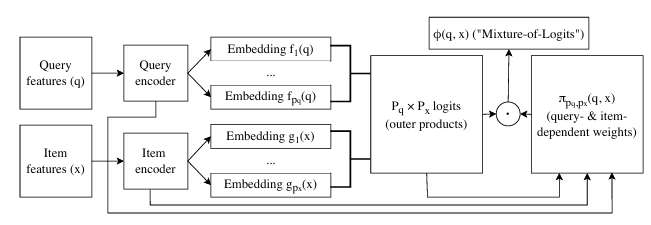
\includegraphics[width=0.7\linewidth]{Figures/mol.png}
	\caption{Mixture of Logits(MoL) learned similarity.}
	\label{Mixture_of_Logits }	
\end{figure}
To determine the similarity between a query and a document, MoL assigns \textbf{adaptive gating weights} \( \pi_p(q,x) \) to the inner products of these low-rank embeddings\citep{zhai2023revisiting}:

\begin{equation}
	\phi(q,x) = \sum_{p=1}^{P} \pi_p(q,x) \langle f_p(q), g_p(x) \rangle
\end{equation}

where \( \pi_p(q,x) \) represents the learned weights for each component, ensuring that their sum equals one. These weights are typically parameterized using a neural network that takes embeddings and their inner products as input features.

To efficiently scale MoL for large datasets and hardware-optimized implementations, the formulation is extended by decomposing the dot products into \textbf{batched outer products} of query-side and document-side embeddings. This decomposition improves computational efficiency, particularly on accelerators like GPUs, by normalizing the embeddings using the \( l_2 \)-norm:\citep{zhai2023revisiting}

\begin{equation}
	\phi(q,x) = \sum_{pq=1}^{P_q} \sum_{px=1}^{P_x} \pi_{pq,px}(q,x) \frac{\langle f_{pq}(q), g_{px}(x) \rangle}{|| f_{pq}(q) ||_2 || g_{px}(x) ||_2}
\end{equation}

Since embedding normalization can be precomputed, both formulations remain interchangeable in practical applications. Furthermore, it is possible to \textbf{decompose any high-rank matrix} into a mixture of logits based on low-rank matrices, demonstrating the flexibility and scalability of this approach in large-scale information retrieval tasks.
\subsection{Algorithm Design}
we introduce an adaptive threshold mechanism
(Dynamic K-Selection for Optimal Retrieval), the MoL framework is employed to refine the
candidate retrieval process. 
\begin{figure}[ht]
	\centering
	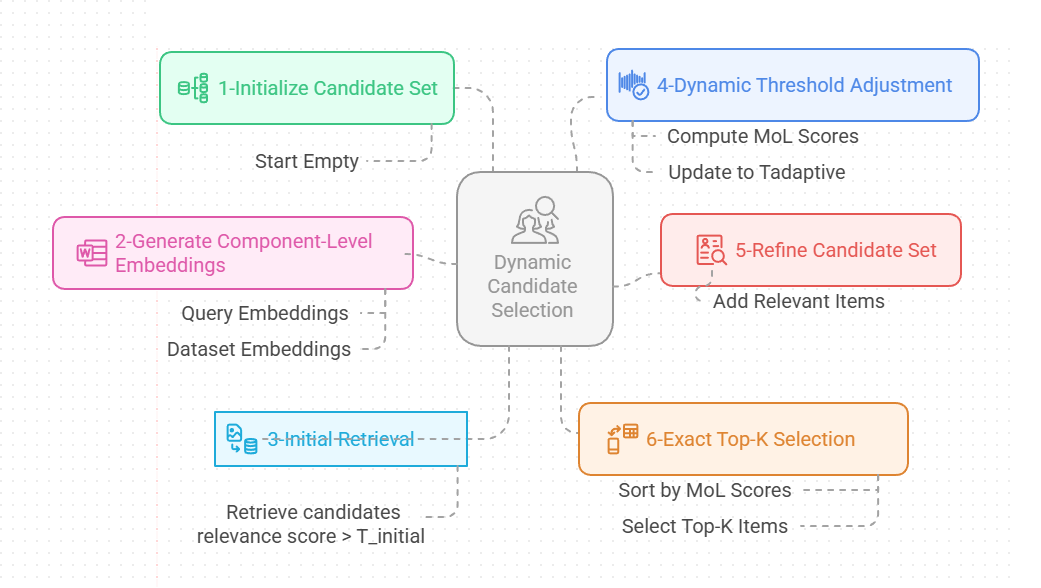
\includegraphics[width=0.7\linewidth]{Figures/propused _solution_steps.png}
	\caption{propused solution steps}
	\label{propused _solution_steps}	
\end{figure}

\noindent

1. \textbf{Component-Level Embeddings}:  
Component-level embeddings are generated for all items in the dataset \(X\). These embeddings facilitate efficient similarity computations during retrieval. Formally,
\begin{equation}
	X_p \leftarrow \{g_p(x) \mid x \in X\}.
\end{equation}

\noindent
2.\textbf{ Initial Candidate Retrieval:} This step involves computing similarity scores between a query representation and item representations for each feature component $p \in P$.  

\begin{equation}
	S_p \gets  \{ \langle f_p(q), g_p(x) \rangle : x \in X_p \}
	\label{eq:initial_retrieval}
\end{equation}
Here, $f_p(q)$ and $g_p(x)$ represent the feature embeddings of the query $q$ and item $x$ for the $p$-th component, respectively. The dot product $\langle f_p(q), g_p(x) \rangle$ measures the relevance of each item $x \in X_p$ with respect to $q$, producing a set of scores $S_p$ .


\noindent
3. \textbf{Dynamic Threshold Adjustment}:  
To improve retrieval quality, \textbf{Mixture of Logits (MoL)} scores are computed for each candidate \(x \in G\). The adaptive gating weights \(\pi_p(q, x)\) allow the algorithm to dynamically adjust the retrieval threshold \(T_{\text{adaptive}}\) based on the MoL scores. The scoring function is defined as:
\begin{equation}
	\phi(q, x) = \sum_{p=1}^{P} \pi_p(q, x) \cdot \langle f_p(q), g_p(x) \rangle.
	\label{similarity_function}
\end{equation}
The adaptive threshold \(T_{\text{adaptive}}\) is set as the minimum score among the candidates:
\begin{equation}
	T_{\text{adaptive}} = \min\{s \mid s \in G\}.
\end{equation}

\noindent
4. \textbf{Refinement and Top-K Selection}:  
Using the adaptive threshold \(T_{\text{adaptive}}\), additional relevant candidates are retrieved, expanding the candidate set \(G'\). This is achieved by including candidates whose scores exceed the threshold:
\begin{equation}
	G' \leftarrow G \cup \{x \mid s_p \geq T_{\text{adaptive}}\}.
\end{equation}
The algorithm then sorts \(G'\) based on MoL scores to select the most relevant top-k candidates.

\noindent
4. \textbf{Exact Top-K Selection}:  
Finally, the candidates in \(G'\) are sorted by their MoL scores, and the exact top-k items are extracted:
\begin{equation}
	G_{\text{final}} = \text{Top-k}(G', \phi(q, x)).
\end{equation}
As shown in Algorithm\ref{ALgo1}, the retrieval process dynamically adjusts the threshold based on MoL scores.



\subsection{Hybrid k-Selection Algorithm Pseudocode}
The following pseudocodeAs shown in Algorithm\ref{ALgo1} outlines our proposed Dynamic K-Selection for Optimal Retrieval algorithm. This method adaptively selects the number of top-k documents retrieved based on query characteristics, enhancing the relevance and efficiency of the retrieval step in our RAG pipeline

\begin{algorithm}
	\caption{Hybrid Exact Top-k with Threshold-Based k Selection}
	\label{ALgo1}
	\textbf{Input:} Query $q$, Set of items $X$, Component-level embeddings: $f_p(q)$, $g_p(x)$ for $p \in P$, $x \in X$, Initial threshold $T_{\text{init}}$ \\
	\textbf{Output:} Exact top $k$ items based on dynamic threshold   selection, $G_{\text{final}}$
	
	\begin{algorithmic}[1]
		
		
		\State Set $G \gets \emptyset$     \Comment{Initial candidate set}
		\For{each component $p \in P$}
		\State $X_p \gets \{g_p(x) \mid x \in X\}$ \Comment{Precompute embeddings}
		\EndFor
		
		\textbf{1. Initial Candidate Retrieval:}
		\For{each component $p \in P$}
		\State Compute dot product scores:  with (eq\eqref{eq:initial_retrieval})
		
		\State Retrieve items with scores $S_p \geq T_{\text{init}}$
		\State Add these items to $G$
		\EndFor
		
		\textbf{2. Adjust k Dynamically:}
		\For{each $x \in G$}
		\State Compute MoL scores $s \gets \phi(q, x)$ using : eq\eqref{similarity_function}
		\State Set $T_{\text{adaptive}} = \min \{s : s \in G\}$
		\EndFor
		
		\textbf{3. Refine Candidate Set with Adaptive k:}
		\State	$G' \gets \emptyset$
		\For{each component $p \in P$}
		\State Retrieve items from $X_p$ with scores $S_p \geq T_{\text{adaptive}}$
		\State Add these items to $G'$
		\EndFor
		
		\textbf{4. Select Exact Top-k Items:}
		\For{each component $p \in P$}
		\State Compute MoL scores for all items in $G'$
		\State Sort $G'$ by MoL scores in descending order
		\State Select the top $k$ items from $G'$ where $k$ is the number of items in $G'$ exceeding $T_{\text{adaptive}}$
		\EndFor
		\State\textbf{ Return:} $G_{\text{final}}$ \Comment{Retrieve Top $k$ items from $G'$}
	\end{algorithmic}
\end{algorithm}

\newpage

\section{Experimental Results}\label{sec3}
In order to measure the effectiveness of our proposed method, we perform a comprehensive evaluation of both the retrieval algorithm and the Mixture-of-Logits (MoL) approach. This assessment focuses on the next-item prediction task, a fundamental challenge in recommendation systems\citep{kang2018selfat},
where the goal is to predict the most relevant item a user will interact with next based on their past interactions. 
\subsection{Dataset Design}
We conducted experiments using two MovieLens datasets : ML-100K and ML-1M \citep{Harper2015}which are widely used benchmarks for evaluating sequential recommendation models as detailed in Table\ref{tab_movielens}.\\
\begin{table}[h]
	\centering
	\renewcommand{\arraystretch}{1.2}
	\begin{tabular}{|l|p{10cm}|}
		\hline
		\textbf{Dataset} & \textbf{Description} \\
		\hline
		\textbf{MovieLens-100K} & 100,000 ratings (1-5 scale) from 943 users on 1,682 movies. \\
		& Each user has rated at least 20 movies. \\
		& Includes user demographic information (age, gender, occupation, zip code). \\
		\hline
		\textbf{MovieLens-1M} & 1,000,209 ratings from 6,040 users on approximately 3,900 movies. \\
		& Data collected from users who joined MovieLens in 2000. \\
		& Represents a larger-scale recommendation scenario. \\
		\hline
	\end{tabular}
	\caption{Summary of MovieLens datasets}
	\label{tab_movielens}
\end{table}

\subsection{Experimental Setup }
For both datasets, We utilize the SASRec architecture as our sequential user encoder, a model renowned for achieving state-of-the-art performance in next-item prediction tasks. This architecture processes the user's historical interaction sequence, generating embeddings that encapsulate the user's preferences at each time step. These embeddings serve as the foundation for predicting the next item in the sequence.

The query \( q \) represents the user's state at a specific time step, derived from their interaction history. In the MoL (Mixture of Logits) framework,\( q \)is transformed into \( Pq \)
embeddings through a multi-layer perceptron (MLP).

For fair comparison, we maintained consistent architectural choices and training conditions across all experiments, We conducted an extensive hyperparameter analysis comparing both approaches (Hybrid+SAS and MoL+SAS) across different architectural configurations:
\subsubsection{Fixed Experimental Configuration}
\begin{itemize}
	\item \textbf{Hardware}: Google Colab with T4 GPU
	\item \textbf{Framework}: TensorFlow
	\item \textbf{Optimizer}: Adam ($\eta=0.001$)
	\item \textbf{Hybrid Specific}: $T_{init}=0.3$ (init threshold)
     
\end{itemize}
For the hybrid algorithm, we initialize the threshold (Tinit) to 0.3 and adaptively adjust it during training. We discuss detailed hyperparameter settings in table \ref{tab:all_results}, table
\subsection{Architectural Variants and Results}

The following tables present our complete experimental results across different model configurations. 
\begin{table}[h]
	\centering
	
	\resizebox{\textwidth}{!}{
		\begin{tabular}{lccccccc}
			\toprule
			\multirow{2}{*}{\textbf{Model}} & 
			\multirow{2}{*}{\textbf{SeqLen}} & 
			\multirow{2}{*}{\textbf{EmbDim}} & 
			\multirow{2}{*}{\textbf{Heads}} & 
			\multicolumn{2}{c}{\textbf{100kMovies}} & 
			\multicolumn{2}{c}{\textbf{1M Movies}} \\
			\cmidrule(lr){5-6} \cmidrule(lr){7-8}
			& & & & Val Loss & Val Acc & Val Loss & Val Acc \\
			\midrule
			Hybrid+SAS & 50 & 128 & 2 & 5.3036 & 0.1584 & 4.5721 & 0.1530 \\
			MoL+SAS & 50 & 128 & 2 & 5.3152 & 0.1582 & 4.5733 & 0.1526 \\
			\addlinespace
			Hybrid+SAS & 128 & 256 & 4 & 3.6364 & 0.4301 & 3.4152 & 0.3680 \\
			MoL+SAS & 128 & 256 & 4 & 3.6374 & 0.4299 & 3.4671 & 0.3627 \\
			\addlinespace
			Hybrid+SAS & 512 & 512 & 4 & 1.2808 & \textbf{0.8120} & 1.0275 & \textbf{0.8350} \\
			MoL+SAS & 512 & 512 & 4 & 1.3050 &\textbf{ 0.8016} & 1.0350 &\textbf{ 0.8276 }\\
			\bottomrule
		\end{tabular}
		
	}
	\caption{Performance Across Configurations}
	\label{tab:all_results}
\end{table}

Both approaches demonstrate significant performance improvements as model capacity increases, with larger configurations consistently delivering better results. For instance, when increasing the model's capacity such as expanding the (Max Sequence Length: 512, Embedding Dimension: 512, Number of Heads: 4, Feed-Forward Dimension: 512) the hybrid algorithm combined with SASRec (Hybrid+SAS) achieves notable gains, particularly in the most resource-intensive setup. On the ML-100K dataset, Hybrid+SAS reaches a score of\textbf{0.8120} compared to the baseline's \textbf{0.8016}, while on ML-1M, it achieves \textbf{0.8350} versus \textbf{0.8276} The ML-1M dataset generally benefits more from increased capacity, with the performance gap between datasets narrowing as the model scales. While smaller configurations provide a balance of efficiency and performance, the largest configuration, despite its higher computational demands, yields the best results, making it suitable for scenarios where resources are not a constraint. Both approaches show similar benefits from scaling, but Hybrid+SAS maintains a consistent edge in performance.


\subsection {Impact of Adaptive k-Variations on Model Performance}
As shown in Figures~\ref{fig:k_changes_100K} and \ref{fig:k_changes_1M}, the value of $k$ fluctuates across epochs for both MovieLens 100K and MovieLens 1M datasets. These variations indicate the adaptive nature of $k$ in response to the dataset characteristics and training progress. In the following section, we analyze how these changes influence model performance.  

\begin{figure}[htbp]
	\centering
	\begin{subfigure}{0.48\textwidth}
		\centering
		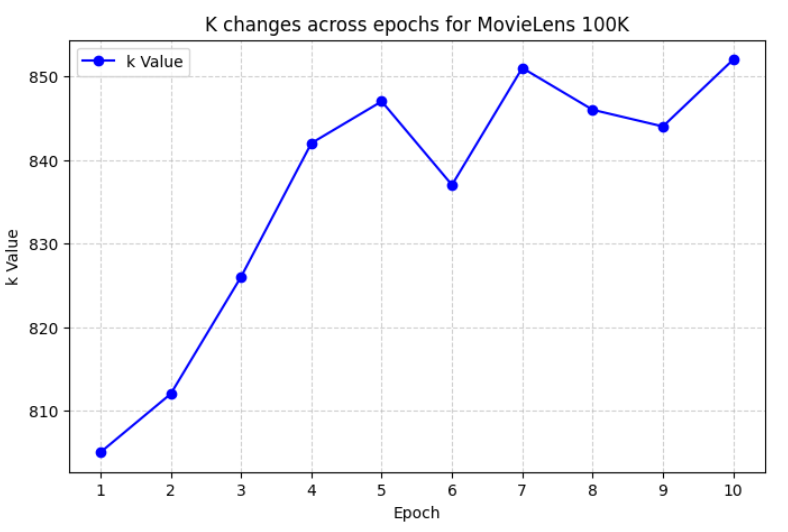
\includegraphics[width=\linewidth]{Figures/CHAGES_OF_K_FOR_100k.png}
		\caption{K changes across epochs for MovieLens 100K}
		\label{fig:k_changes_100K}
	\end{subfigure}
	\hfill
	\begin{subfigure}{0.48\textwidth}
		\centering
		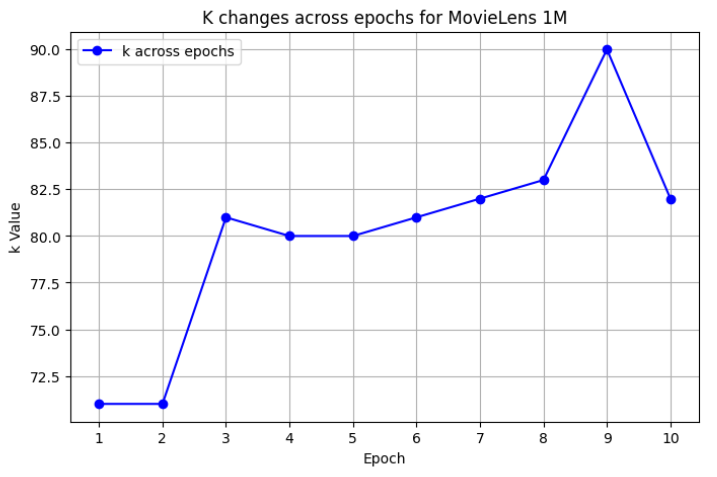
\includegraphics[width=\linewidth]{Figures/chnages_inK_for_1M.png}
		\caption{K changes across epochs for MovieLens 1M}
		\label{fig:k_changes_1M}
	\end{subfigure}
	\caption{Comparison of K changes across epochs for different datasets}
	\label{fig:k_changes}
\end{figure}
the value of K changed dynamically during training, with different behaviors. For the MovieLens 100K dataset, K showed a steady increase across epochs, whereas for the MovieLens 1M dataset, K began at a lower value, experienced fluctuations, peaked, and then stabilized. This indicates that the larger dataset necessitated more adaptive adjustments in retrieval compared to the smaller dataset.\\
Figure~\ref{histo_p} summarizes the performance of our hybrid algorithm compared to the MoL-based approach on the MovieLens 100K and 1M datasets, both tested using a Max Sequence Length of 50, an Embedding Dimension of 128, 2 Attention Heads, a Feedforward Dimension of 128, a Batch Size of 128, and trained for 10 epochs . \\
\begin{figure}[ht]
	\centering
	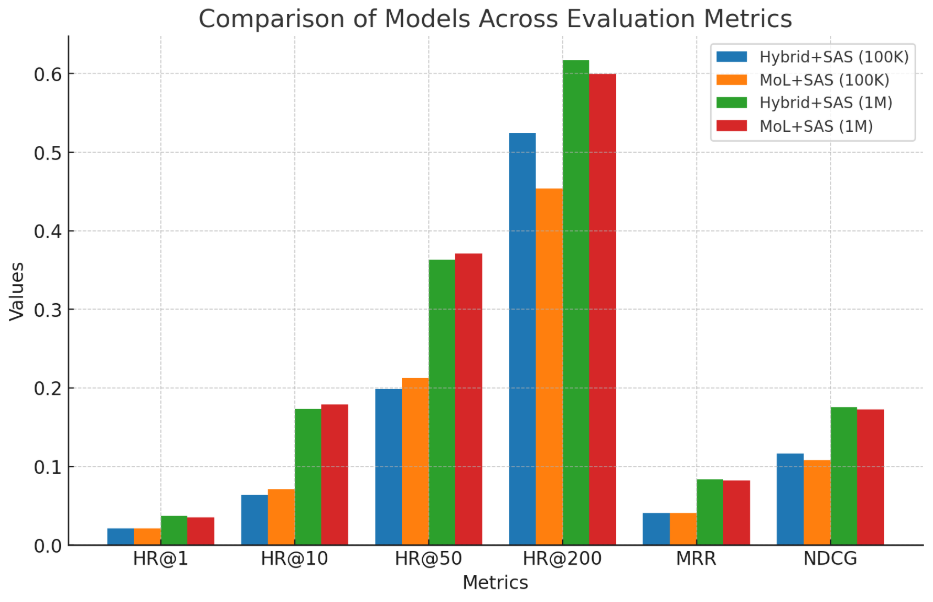
\includegraphics[width=0.7\textwidth]{Figures/HISTOGRAM.png}
	\caption{Comparison of Models Across Evaluation Metrics}\label{histo_p}
\end{figure}
The variations in K help explain the performance differences seen in the fig \ref{histo_p}. The Hybrid+SAS model applied to the MovieLens 1M dataset, which exhibited more dynamic changes in K achieved higher HR@50(0.3631) and HR@200(0.6170) scores, reflecting better long-range recommendation quality. The fluctuations in K in the 1M dataset likely allowed the model to balance exploration and precision, improving its overall ranking performance.

On the other hand, the more gradual K increase in the 100K dataset resulted in relatively lower scores, suggesting that a static or overly conservative 
K selection might limit retrieval effectiveness.

Additionally, the MoL+SAS model achieved better performance than Hybrid+SAS in HR@10 for both datasets. This aligns with the observation that MoL+SAS tended to retrieve fewer but more relevant items at shorter ranking positions. This behavior can be attributed to how K evolved during training?smaller K values in earlier epochs likely enabled MoL+SAS to maintain higher precision at shorter ranks.
These findings highlight the importance of dynamically tuning K based on dataset characteristics to optimize recommendation effectiveness.


The results demonstrate that the Hybrid Exact Top-k algorithm effectively leverages both sequential user behavior and item metadata to improve recommendation quality. The adaptive MoL threshold allows the model to dynamically refine candidate items during training, leading to better performance. The improvements are consistent across both datasets, highlighting the robustness of our approach.\\ 
\section{Conclusion}

The selection of $k$ in retrieval plays a pivotal role in balancing relevance, efficiency, and computational cost. Throughout this chapter, we explored how different approaches—static, dynamic, and hybrid—impact retrieval performance and generation quality. While static selection provides consistency, it lacks adaptability to varying query complexities. Dynamic methods introduce flexibility but come with computational overhead, whereas hybrid strategies aim to balance both. The Hybrid Exact Top-$k$ with Threshold-Based $k$ Selection method offers an advanced solution by leveraging adaptive weighting to enhance ranking effectiveness.

Although this method has shown promising results in large-scale retrieval scenarios, its integration into our Arabic legal RAG agent was not feasible due to the limited size and scope of our dataset, which contains only around 100 manually constructed cases, many of which are not fully accessible or diverse. The effectiveness of threshold-based $k$ selection becomes more apparent when applied to larger and more representative datasets. Therefore, we consider this a valuable avenue for future work—once the dataset is expanded, implementing and testing this dynamic approach could significantly enhance the performance and adaptability of our Agent.

Ultimately, an effective $k$-selection strategy is essential for optimizing retrieval, ensuring both efficiency and high-quality results in knowledge-augmented applications.
